\documentclass[svgnames]{article}   	% use "amsart" instead of "article" for AMSLaTeX format
%\geometry{landscape}                	% Activate for rotated page geometry

%\usepackage[parfill]{parskip}    		% Activate to begin paragraphs with an empty line rather than an indent

\usepackage{graphicx}				          % Use pdf, png, jpg, or eps§ with pdflatex; use eps in DVI mode
\setcounter{secnumdepth}{4}
\setcounter{tocdepth}{4}
%maths							                  % TeX will automatically convert eps --> pdf in pdflatex		
\usepackage{amssymb}
\usepackage{amsmath}
\usepackage{esint}
\usepackage{geometry}

%pgfplots
\usepackage{pgfplots}

%images
\graphicspath{{/Users/devaldeliwala}}					          % Activate to set a image directory 

%tikz
\usepackage{pgfplots}
\pgfplotsset{compat=1.15}
\usepackage{comment}
\usetikzlibrary{arrows}
\usepackage[most]{tcolorbox}

%Figures
\usepackage{float}
\usepackage{caption}
\usepackage{lipsum}


\title{5B - Introductory Electromagnetism, Waves, and Optics}
\author{deval deliwala}
%\date{}							                % Activate to display a given date or no date

\begin{document}
\maketitle
%\section{}
%\subsection{}
\tableofcontents 					           % Activate to display a table of contents
\newpage

\noindent \textbf{Jan 17} 
\hrule
\section{Maxwell's Equations}

\begin{align*} 
      &\nabla \cdot \vec{E} = \frac{\rho}{\varepsilon_0}      \\  
      &\nabla \times \vec{B} = \mu_0\vec{J} + \mu_0\varepsilon_0 \frac{\partial
      \vec{E}}{\partial t} \\
      &\nabla \times \vec{E} = - \frac{\partial \vec{B}}{\partial t} \\
      &\nabla \cdot \vec{B} = 0
\end{align*}
\vspace{5px}

The goal of this course will be to understand Maxwell's Equations, and the
unison between the electric and magnetic field. 
\vspace{5px}

\begin{tcolorbox}[colback = red!5!white, colframe = red!50!black, title
  = Lorent'z Force eq]
  \[
  \vec{F} = q\vec{E} + q\vec{v} \times \vec{B}
  \]
\end{tcolorbox}
\vspace{5px}
\begin{tcolorbox}[colback = blue!5!white, colframe = blue!50!black, title
  = Rules]
  
  1. Charge in nature is quantized in units of $e$ \\
  2. Charge is conserved \\
  3. Charge has 2 types: $\pm$

\end{tcolorbox}
\vspace{5px}

$\vec{E}$ and $\vec{B}$ are \textit{vector fields}. This means $\vec{E}$ is
a function of every point in space: $\vec{E}(x,y,z)$

\vspace{5px}\[
  \vec{E}(r) = E_x(x,y,z)\hat{i} + E_y(x,y,z)\hat{j} + E_z(x,y,z)\hat{k}
\] \vspace{5px}
\newpage
$\nabla$ is a vector operator: 

\vspace{5px} \[
  \frac{\partial }{\partial x} \hat{i} + \frac{\partial }{\partial y} \hat{j}
  + \frac{\partial }{\partial x} \hat{k}
\] \vspace{5px}

\begin{tcolorbox}[colback = red!5!white, colframe = red!50!black, title
  = Vector Operations]
  
  \[
    \vec{A}\alpha \rightarrow \vec{B}
  \]
  \[
    \vec{A} \cdot \vec{B} \rightarrow \alpha
  \]
  \[
    \vec{A} \times \vec{B} \rightarrow \vec{C}
  \]

\end{tcolorbox}
\vspace{5px}

Consider a scalar field: $\varphi(\vec{r})$
\begin{align*}
&d\varphi = \varphi(r + dr) - \varphi(r) \\
&d\varphi = \frac{\partial \varphi(x,y,z)}{\partial x}dx + \frac{\partial
\varphi(x,y,z)}{\partial y}dy + \frac{\partial \varphi(x,y,z)}{\partial z}dz\\
&d\vec{r} = \hat{i}dx + \hat{y}dy + \hat{z}dz
\end{align*}
\begin{tcolorbox}
\[
  d\varphi = \nabla \varphi(\vec{r}) \cdot d\vec{r}
\]
\end{tcolorbox}
\vspace{5px}

$\nabla \varphi$ = "gradient of $\varphi$. " Also $\nabla \cdot \vec{E}
= \frac{\partial E_x}{\partial x}+ \frac{\partial E_y}{\partial y}
+ \frac{\partial E_z}{\partial z}$. This is known as the \textbf{divergence} of
$\varphi$. 
\vspace{10px}

The \textbf{curl} of $\varphi$ is equal to 

\vspace{5px} \[
\begin{vmatrix}
  \hat{i} & \hat{j} & \hat{k} \\
  P & Q & R \\
  \frac{\partial }{\partial x} & \frac{\partial }{\partial y} & \frac{\partial
  }{\partial z}  
\end{vmatrix}
\] \vspace{5px}
\[
  \rho = \text{charge density} = \frac{\text{number of particles} q}{dV} = nq
\] \vspace{5px}
where $n = \frac{\text{number of particles}}{dv}$


\vspace{5px} \[
  \vec{J} = \text{current density}
\] \vspace{5px}

\section{Statics}

\begin{tcolorbox}[colback = red!5!white, colframe = red!50!black, title
  = Equations of Electrostatics]
  
  \[
    \nabla \cdot \vec{E} = \frac{\rho}{\varepsilon_0}
  \]
  \[
    \nabla \times \vec{E} = 0
  \] 
  
\end{tcolorbox}

\begin{tcolorbox}[colback = blue!5!white, colframe = blue!50!black, title
  = Equations of Magnetostatics]
  
  \[
    \nabla \cdot \vec{B} = 0
  \]
  \[
    \nabla \times \vec{B} = \mu_0\vec{J}
  \] 

\end{tcolorbox}

\subsection{Flux}
\vspace{5px}
"Flux" = Flow 

\vspace{10px} 

Consider a fluid flow with a velocity vector field $\vec{v}(\vec{r})i$, flowing
into a small aperture defined by $\hat{n}\,d\vec{a}$, where  $\hat{n}$ is the
unit normal vector to the aperture, and $d\vec{a}$ is the area. 

\[
  d\Phi = \vec{v} \cdot d\vec{a}
\]

Relating to the Electric field, 

\[
  d\Phi_E = \vec{E}(\vec{r}) \cdot d\vec{a}
\] 
\[
  \int_S d\Phi_E = \Phi_E = \int_S \vec{E}(\vec{r}) \cdot d\vec{a}
\]\vspace{5px}

Green's, Gauss's, Divergence Theorem

\[
  \int_S \vec{E} \cdot d\vec{a} = \iiint_S \nabla \cdot \vec{E}(\vec{r}) \, d^3
  r
\]

\newpage
\noindent \textbf{Jan 19} \hrule
\vspace{5px} \[
  \Phi = \oint_S \vec{E}(\vec{r}) \cdot d\vec{a} = \iiint_V d^3r \, \nabla \cdot
  \vec{E}(\vec{r}) \rightarrow \text{Divergence Theorem}
\] \vspace{5px}


%1
% flux from two sides of a cube

\begin{figure}[htb!]
  \centering
    \includegraphics[width = 10cm]{screenshot 28.png}
    \caption{Flux from two sides of cube}
\end{figure}
\vspace{5px}


\begin{align*}
  d\Phi_{12} &= \vec{E}(x,y,z) \cdot d\vec{a_1} + \vec{E}(x+dx, y,z) \cdot
  d\vec{a_2} \hspace{10px} | \hspace{10px} 
   d\vec{a_1} = -\hat{i}dydz, d\vec{a_2} = \hat{i}dydz\\ \\
  d\Phi_{12} &=[ E_x (x + dx, y,z) -  E_x(x,y,z) ] \, dydz\\
  d\Phi_{12} &= \left[\frac{\partial E_x(x,y,z)}{\partial x} \, dx\right]
  dydz\\ \\
\text{Since } dv = dxdydz, \\ \\
  d\Phi_{12} &= \frac{\partial E_x(x,y,z)}{\partial x}  \cdot d^3v\\
  d\Phi_{tot} &= d\Phi_{12} + d\Phi_{34} + \dots\\
              &= \left( \frac{\partial E_x}{\partial x}  + \frac{\partial E_y}{\partial y}
  + \frac{\partial E_z}{\partial z} \right) \, d^3 r \\
  d\Phi_{tot} &= \nabla \cdot \vec{E}(\vec{r}) \, d^3 r\\\\
  \nabla \cdot \vec{E} &= \frac{d \Phi}{d^3 r} \\
  \nabla \cdot E &= \frac{\text{flux}}{\text{volume}}
\end{align*} 
\vspace{5px}

%2
% flux from the boundary of the surface is equivalent to adding the flux of
% every $dV$ insidei

\begin{figure}[htb!]
  \centering
    \includegraphics[width = 10cm]{screenshot 29.png}
    \caption{Flux from the boundary surface is equal to adding the flux of
    every $dV$ inside}
\end{figure}




\subsection{Divergence Theorem}

\begin{tcolorbox}	
  \[ 
  \iiint \nabla \cdot \vec{E} (\vec{r} ) \, d^3r = \oint_S \vec{E} \cdot d\vec{a}
  \]
\end{tcolorbox}	

\vspace{5px} \[
\iiint \frac{\rho(\vec{r})}{\epsilon_0} d^3r = \oint \vec{E}(\vec{r} ) \cdot
d\vec{a}
\] \vspace{5px}


\begin{tcolorbox}[colback = red!5!white, colframe = red!50!black, title = Gauss' Law]
  \[
    \Phi = \frac{Q}{\varepsilon_0}
  \]
\end{tcolorbox}

%3
% flux from positive charge is positive (source), flux from negative charge is
% negative (sink)

\begin{figure}[H]
  \centering
    \includegraphics[width = 8cm]{screenshot 30.png}
    \caption{Flux from positive charge is positive (source), flux from negative
    charge is negative (sink)}
\end{figure}


\subsection{Coulomb's Law}
\vspace{5px}

%4
% electric field from a sphere is directly outward and has same magnitude due to symmetry

\begin{figure}[htb!]
  \centering
    \includegraphics[width = 8cm]{screenshot 31.png}
    \caption{Electric field from a sphere is directly outward and has the same
    magnitude due to symmetry}
\end{figure}

\subsection{Electric Field of Point Charge}
\vspace{5px}
\begin{align*}
\vec{E} (\vec{r} ) \propto \hat{r} \\
\Phi &= \frac{Q}{\epsilon_0}\\
E(r) \cdot 4\pi r^2 &= \frac{Q}{\epsilon_0}\\
\vec{E}(\vec{r} ) &= \hat{r}\frac{Q}{4\pi \epsilon_0 r^2}
\end{align*}

%5
%diagram of coulomb's law
\begin{figure}[H]
  \centering
    \includegraphics[width = \linewidth]{screenshot 32.png}
    \caption{Diagram of Coulomb's Law}
\end{figure}



\begin{tcolorbox}[title = Coulomb's Law]
\[
  \vec{F_{21}} = q_2 \vec{E_1}(P_2) = \frac{q_2q_1}{4 \pi \epsilon_0 r^2}
  \hat{r_{21}}
\]
\end{tcolorbox}

The force is proportional to the product of the charges, and inversely
proportional to the square of the distance, and directed along the line between
the charge, and directed along the line between the charges. Attractive for
opposite signs of charge, and vice versa. 

%6
%comparison between $F_g$ and $F_c$ i

\begin{figure}[H]
  \centering
    \includegraphics[width = 8cm]{screenshot 33.png}
    \caption{Comparison between $F_g$ and $F_c$}
\end{figure} 

\newpage
\textit{ \textbf{Jan 19 Summary}} 
\vspace{5px} \[
  \iiint_V \nabla \cdot \vec{E} (\vec{r} ) \, dxdydz = \oint_S \vec{E} \cdot
  d\vec{a}
\] \vspace{5px}
\vspace{5px} \[
  \Phi = \frac{Q}{\epsilon_0} \rightarrow \vec{E}_{\text{point charge}}
  = \frac{Q}{4\pi r^2 \epsilon_0}
\] \vspace{5px}
\newpage
\noindent \textbf{Jan 24} \hrule
\vspace{10px} 

\begin{tcolorbox}[colback = red!5!white, colframe = red!50!black, title
  = Calculating $\vec{E}$ for arbitrary $\rho(\vec{r)}$]
  
  Superposition: $\nabla \cdot \vec{E} = \frac{\rho}{\epsilon_0}$, works
  because Maxwell's Equation are linear.

  \begin{align*}
    &\nabla \cdot \vec{E_1} = \frac{\rho_1}{\varepsilon_0} \\
    &\nabla \cdot \vec{E_2} = \frac{\rho_2}{\varepsilon_0} \\\\
    &\nabla \cdot (\vec{E_1} + \vec{E_2}) = \frac{\rho_1 + \rho_2}{\varepsilon_0}
  \end{align*}

  Proved $\nabla \cdot \vec{E_T} = \frac{\rho_T}{\varepsilon_0}$
\end{tcolorbox}

%1
%volumes of charge
\begin{figure}[htb!]
  \centering
    \includegraphics[width = 7cm]{screenshot 41.png}
    \caption{volumes of charge}
\end{figure}



%2
%system of charges, notation of vectors


\begin{figure}[htb!]
  \centering
    \includegraphics[width = 5cm]{screenshot 42.png}
    \caption{system of charges}
\end{figure}

\begin{figure}[htb!]
  \centering
    \includegraphics[width = 8cm]{screenshot 43.png}
    \caption{notations of vectors, $\vec{r}, \vec{r_1}, \vec{r} - \vec{r_1}$}
\end{figure}


\begin{tcolorbox}[colback = blue!5!white, colframe = blue!50!black, title
  = System of point charges]

Therefore the field at $P$ is

\[
\vec{E_1}(\vec{r}) = \frac{q_1}{4\pi\varepsilon_0}\frac{1}{|\vec{r}
- \vec{r_1}|^2} \cdot \frac{(\vec{r} - \vec{r_1})}{|\vec{r}- \vec{r_1}|}
= \frac{q_1}{4\pi\varepsilon} \frac{(\vec{r}-\vec{r_1})}{|\vec{r}  - \vec{r_1}
|^3}
\]
Superposition: 

\[
\vec{E}(\vec{r} ) = \sum_i \frac{q_i}{4\pi\varepsilon_0} \frac{(\vec{r}
- \vec{r_1} )}{|\vec{r} - \vec{r_1} |^3}
\]
\end{tcolorbox}

%3
%volume charge distribution, $dq = \rho(r) d^3 v$

\begin{figure}[htb!]
  \centering
    \includegraphics[width = 8cm]{screenshot 44.png}
    \caption{volume charge distribution, $dq = \rho(r) d^3 v$}
\end{figure}

\begin{figure}[htb!]
  \centering
    \includegraphics[width = 3cm]{screenshot 45.png}
    \caption{using symmetry to determine component of $\vec{E}$}
\end{figure}



\begin{tcolorbox}	
  
  \[
  \vec{E}(\vec{r}) = \frac{1}{4\pi\varepsilon_0} \int d^3r'
  \frac{\rho(\vec{r}')(\vec{r} - \vec{r}' }{|\vec{r} - \vec{r}'|^3}
  \]
  \[
    \nabla \cdot \vec{E} = \frac{\rho}{\varepsilon_0}
  \]

\end{tcolorbox}	


\subsection{Gauss's Law + Symmetry} 

%4
%different Gauss' law symmetries, symmetry of sphere of charge

\begin{figure}[H]
  \centering
    \includegraphics[width = 10cm]{screenshot 46.png}
    \caption{different Gauss's Law symmetries, symmetry of a sphere of charge}
\end{figure}


\paragraph{Symmetry of cylinder of charge}

%5
%symmetry of cylinder - field has to be radial

\begin{figure}[H]
  \centering
    \includegraphics[width = 10cm]{screenshot 47.png}
    \caption{symmetry of a cylinder of charge}
\end{figure}


\paragraph{Symmetry of plane of charge}

%6
%symmetry of plane - mirror symmetry

\begin{figure}[H]
  \centering
    \includegraphics[width = 8cm]{screenshot 48.png}
    \caption{symmetry of a plane -- mirror symmetry}
\end{figure}



\paragraph{Using Gauss's Law symmetry}

\textbf{Problem. Uniform Sphere of Charge}  
  
\begin{figure}[H]
  \centering
    \includegraphics[width = 7cm]{screenshot 49.png}
    \caption{uniform sphere of charge, inside and outside the radius}
\end{figure}



\begin{align*}
  \text{Gauss's Law} \\\\
  &\oint_S = \vec{E} \cdot d\vec{a} = \frac{Q}{\varepsilon_0}\\\\
  \text{Outside Surface}\\
  &E(r) \cdot 4\pi r^2 = \frac{\rho_0 \frac{4\pi
  r^3}{3}}{\varepsilon_0 } \\
  &E(r) = \frac{\rho_0 R^3}{3\varepsilon_0 r^2} = \frac{Q}{4\pi r^2
  \varepsilon_0} \\\\
  \text{Inside Surface} \\
  &E(r) \cdot 4\pi r^2 = \frac{Q}{\varepsilon_0} \cdot \left(\frac{r}{R}\right)^3
\end{align*}

\begin{tcolorbox}	
    Outside: 
    \[E(r) = \frac{Q}{4\pi r^2 \varepsilon} \]
  Inside: 
  \[E(r) = \frac{Q}{4\pi \varepsilon} \frac{r}{R^3} \]
\end{tcolorbox}	


%7
%graph of $E(r) v. $r$ for a spherical charge distribution

\begin{figure}[H]
  \centering
    \includegraphics[width = 8cm]{screenshot 50.png}
    \caption{graph of $E(r)$ v.  $r$ for a spherical charge distribution}
\end{figure}





\paragraph{Lower Dimensional Charge Distributions}

%8
%1 and 2 dimensional charge distributions - $\sigma$ and $\lambda$

\begin{figure}[H]
  \centering
    \includegraphics[width = 6cm]{screenshot 51.png}
    \caption{1 and 2 dimensional charge distributions - $\sigma$ and $\lambda$}
\end{figure}




\paragraph{Applying Gauss's Law to a Plane of Charge}

%9
%gaussian surface of a plane of charge

\begin{figure}[H]
  \centering
    \includegraphics[width = 10cm]{screenshot 52.png}
    \caption{gaussian surface of a plane of charge}
\end{figure}



\begin{align*}
  2E(r)A &= \frac{\sigma A}{\varepsilon_0} \\
  E &= \frac{\sigma}{\varepsilon_0} 
\end{align*}

\newpage
\noindent \textbf{Jan 26} \hrule
\vspace{10px} 
\subsection{Visualizing the Electric Field}
%1

\begin{figure}[H]
  \centering
    \includegraphics[width = 11cm]{screenshot 66.png}
    \caption{visualizing electric field lines}
\end{figure}



%2
\begin{figure}[H]
  \centering
    \includegraphics[width = 10cm]{screenshot 67.png}
    \caption{area density of field lines}
\end{figure}



\subsection{Energy, Work, and Electrostatic Potential}

\paragraph{Work-Energy Theorem} 

Consider a charged particle, moving in a force field $\vec{F}(r)$
%3
\begin{figure}[H]
  \centering
    \includegraphics[width = 6cm]{screenshot 68.png}
    \caption{trajectory of $\vec{r}(t)$ }
\end{figure}



%trajectory of the charged particle, with a small $d\vec{r} $
\begin{align*}
  \vec{F}(\vec{r}) &= m \frac{d \vec{v}}{d t} \\  
  \vec{F}(\vec{r}) \cdot d\vec{r} &= m \frac{d \vec{v}}{d t} \cdot d\vec{r}
  \hspace{20px} \frac{d \vec{r} }{d t} = \vec{v} \\ 
                   &= m \frac{d \vec{v}}{d  t} \cdot \vec{v}dt = m d\vec{v} \cdot \vec{v} 
\end{align*}

\begin{align*}
  d(\vec{v} \cdot \vec{v}) &\rightarrow \text{Chain rule} \rightarrow \vec{v}
  \cdot d\vec{v} + d\vec{v} \cdot \vec{v} = 2 d\vec{v} \vec{v} \\\\
  d\vec{v} \cdot \vec{v} &= \frac{1}{2}dv^2 \\
  \vec{F}\cdot d\vec{r} &= \frac{m}{2} dv^2 
\end{align*}

\vspace{5px} \[
  \int_{r_a}^{r_b} \vec{F}\cdot d\vec{r} = \frac{m}{2}\int_{r_a}^{r_b} d(v)
  = \frac{m}{2}\left[v^2(r_b) - v^2(r_a) \right]
\] \vspace{5px}

Therefore, $\int_{\vec{r_a}}^{\vec{r_b}} \vec{F}(\vec{r}) \cdot d\vec{r}
= $ Work done by the force. 
\vspace{5px}
\begin{tcolorbox}
\[
  \int_{\vec{r_a}}^{\vec{r_b}} \vec{F}(\vec{r)} \cdot d\vec{r} = \Delta KE 
\]
\end{tcolorbox}
%4
%conservative force fields

\begin{figure}[H]
  \centering
    \includegraphics[width = 9cm]{screenshot 69.png}
    \caption{conservative force fields}
\end{figure}



%5
%deriving conservative force field from Lorentz's Law

\begin{figure}[H]
  \centering
    \includegraphics[width = 12cm]{screenshot 70.png}
    \caption{deriving conservative force field from Lorentz's Law}
\end{figure}



%6
%intuition for conservativeness

\begin{figure}[H]
  \centering
    \includegraphics[width = 10cm]{screenshot 71.png}
    \caption{intuition for conservative news}
\end{figure}

\textbf{Revision}

\begin{align*}
  W_{ab} = q\int_{\vec{r_a}}^{\vec{r_b}} \vec{E}(\vec{r}) \cdot d\vec{r}
  = q\int_{P_1}^{P_2} \vec{E} \cdot d\vec{r}  
\end{align*}

\[
  W_{ab}^{ext} = \text{work done to move a particle on a trajectory in the
  presence of a force field}
\]

\vspace{5px} \[
  W_{ab}^{ext} = -q\int_{P_1}^{P_2} \vec{E}(\vec{r}) \cdot d\vec{r} 
\] \vspace{5px}
\subsection{Electric Potential} 

Define $\varphi(r_a, r_b)$

\vspace{5px} \[
  \varphi(\vec{r_a}, \vec{r_b}) = -\int_{r_a}^{r_b} \vec{E}(\vec{r}) \cdot
  d\vec{r} 
\] \vspace{5px}
\[
  \varphi = \int_{r_a}^{r_b} d\varphi = \varphi(r_b) - \varphi(r_a) 
\]
\vspace{5px} \[
  W_{ab}^{ext} = q[\varphi(r_b) - \varphi(r_b)] \hspace{20px} \text{relation
  between potential and work}
\] \vspace{5px}

\paragraph{Conservation of Energy}

\begin{align*}
  W_{ab} = K_b - K_a  &= -W_{ab}^{ext} = q[\varphi(r_a) - \varphi(r_b)] \\\\
  K_b + q\varphi(r_b) &= K_a + q\varphi(r_a) \hspace{20px} \text{Conservation of
  Energy} 
\end{align*}

\begin{tcolorbox}[title = Conservation of Energy]

  \[
  K_b + q\varphi(r_b) = K_a + q\varphi(r_a)
  \]

\end{tcolorbox}

\begin{figure}[H]
  \centering
    \includegraphics[width = \linewidth]{screenshot 72.png}
    \caption{Analogy with Gravity}
\end{figure}

\newpage

\noindent \textbf{Jan 31} \hrule
\vspace{10px}
\paragraph{Overview of Last Lecture} 

\paragraph{Work, Energy, and Potential Road Map}

Work Energy Theorem \\ 
(1)
\[
  \int_{\vec{r_a}}^{\vec{r_b}} \vec{F}(\vec{r}) \cdot d\vec{r} = K_b - K_a 
\]

(2) \hspace{10px} This integral must be independent of path, also known as conservative force
field. \\\\

(3) \hspace{10px} Define $dU(r) = - \vec{F} \cdot d\vec{r}$. This is the work one must do to
overcome the Force field and move the particle along some trajectory from $r$
to $dr$ \\\\

(4) 

\[
  \int_{\vec{r_a}}^{\vec{r_b}} dU(\vec{r}) = U(\vec{r_b}) - U(\vec{r_b})
  = - \int_{r_a}^{r_b} \vec{F}(\vec{r}) \cdot d\vec{r} = K_a - K_b
\]
along \textbf{any} path

\vspace{5px} \[
U(\vec{r_b} - U(\vec{r_a}) = K_a - K_b   
\] \vspace{5px}

(5) \hspace{10px} Rearranging terms you develop \textit{Conservation of Energy} 

\[
U(\vec{r_b}) + K_b = U(\vec{r_a}) + K_a  
\]

(6) \hspace{10px}
\[
  U(\vec{r_b}) - U(\vec{r_a}) = -q \int_{r_a} \vec{E} \cdot d\vec{r}  
\]

(7) \hspace{10px} Define  
\[
\varphi(\vec{r_b}) - \varphi(\vec{r_a})
= \frac{1}{q} [U(\vec{r_b}) - U(\vec{r_a})]  
\]

(8) 


\begin{tcolorbox}	
  
  \[
    \varphi(\vec{r_b}) - \varphi(\vec{r_a}) = -\int \vec{E} \cdot d\vec{r}   
  \]
  
  

\end{tcolorbox}	
\vspace{5px}

(9) \hspace{10px} Only potential differences are physically observable


\subsection{Visualizing $\varphi(\vec{r})$}

%1
\begin{figure}[H]
  \centering
    \includegraphics[width = 7cm]{screenshot 84.png}
    \caption{Equipotential Contours}
\end{figure}




\begin{align*}
  &d\varphi(\vec{r}) = - \vec{E} \cdot \vec{r} \\
  &d\vec{r}_\perp \perp \vec{E}(\vec{r}) \\
  &d\varphi(\vec{r}) = \vec{E}(\vec{r}) \cdot d\vec{r}_\perp = 0 
\end{align*}

\paragraph{Potential of a point charge $q$}

%2
\begin{figure}[H]
  \centering
    \includegraphics[width = 7cm]{screenshot 85.png}
    \caption{Equipotential Spheres}
\end{figure}



\begin{align*}
  \vec{E}(\vec{r}) = \frac{q}{4\pi\varepsilon_0 r^2} \hat{r} \\
  \varphi(\vec{r}_b) - \varphi(\vec{r}_a) &= -\int_{\vec{r_a}}^{\vec{r_b}}
  \vec{E}(\vec{r}) \cdot d\vec{r} \\
                              &= \frac{q}{4\pi\varepsilon_0}\int_{r_a}^{r_b}\frac{1}{r^2}dr \\
  \varphi(r_b) - \varphi(r_a) = \frac{q}{4\pi\varepsilon_0} \frac{1}{r}
  \Big|_{r_a}^{r_b} = \frac{q}{4\pi\varepsilon}\left(\frac{1}{r_b}
    - \frac{1}{r_a} \right)
\end{align*}

Choose $r_a = \infty$ 

\[
  \varphi(r_b) - \varphi(\infty) = \frac{q}{4\pi\varepsilon r}
\]

Free to choose $\varphi(\infty) = 0$ 

\vspace{5px}
\begin{tcolorbox}
  \[
  \varphi(r) = \frac{q}{4\pi\varepsilon_0 r} = \frac{1}{4\pi\varepsilon_0}
  \frac{q}{r}
  \]
\end{tcolorbox}
\vspace{5px}

The difference in potential energy of a particle between two points depends on
the sign of the charge. Potential is the potential energy divided by the
charge. \\


A word about units. 

\begin{align*}
  &\text{Work} = \text{Joules} \\
  &q = \text{Coulombs} \\
  &\varphi = \frac{\text{Joules}}{\text{Coulombs}} = \text{Volt}
\end{align*}
\hrule
\vspace{10px} 

\begin{align*}
  &d\varphi(r) = \vec{E} \cdot d\vec{r} \\
  &d\varphi(r) = \nabla \varphi(r) \cdot d\vec{r} \\\\
  &\vec{E}(r) = -\nabla\varphi(r)
\end{align*}

\subsection{Potential of arbitrary charge distributions}

General Math Problem 

\begin{itemize}
  \item $\vec{E}(\vec{r}) = -\nabla \varphi(\vec{r})$
  \item Maxwell  $\nabla \cdot \vec{E} = \frac{\rho}{\varepsilon_0}$
\end{itemize}

\[
  \nabla \cdot \nabla \varphi(\vec{r}) = -\frac{\rho(\vec{r})}{\varepsilon_0}
  = \nabla^2 \varphi(\vec{r})
\]
\[
  \nabla^2 \varphi = \nabla \cdot \nabla \varphi = \left( \frac{\partial^2 \varphi}{\partial
    x^2} + \frac{\partial^2 \varphi}{\partial y^2} + \frac{\partial^2
    \varphi}{\partial z^2} \right) 
\]

\begin{tcolorbox}[title = Poisson's Equation]

  \[
    \nabla^2 \varphi(\vec{r}) = -\frac{\rho(\vec{r})}{\varepsilon_0}
  \]

\end{tcolorbox}

Charge-free region of space: $\nabla^2 \varphi(\vec{r}) = 0$ --- Laplace's
Equation

\[
  \nabla^2 \text{ is known as the Laplacian Operator}
\] \vspace{10px} 

%3
%potential at a point P from a volume charge a distance $\vec{r'} - \vec{r}$
%away
\begin{figure}[H]
  \centering
    \includegraphics[width = 12cm]{screenshot 86.png}
    \caption{potential at a point $P$ from a volume charge a distance  $\vec{r'}
    - \vec{r}$ away}
\end{figure}


\textbf{ \textit{Example}}: Potential of a uniformly charged disk on the
symmetry of axis 

%4

\begin{figure}[H]
  \centering
    \includegraphics[width = 6cm]{screenshot 87.png}
    \caption{A point on the $z$ axis experiences a net vertical electric field}
\end{figure}



\begin{align*}
  \varphi(\vec{r}) = \frac{1}{4\pi\varepsilon_0} \iint d^2 r'
  \frac{\sigma(\vec{r'})}{|\vec{r'} - \vec{r}|}
= \frac{\sigma}{4\pi\varepsilon_0} \iint d^2 r' \frac{1}{|\vec{r'} - \vec{r}|} 
\end{align*}

%5
\begin{figure}[H]
  \centering
    \includegraphics[width = 9cm]{screenshot 88.png}
    \caption{calculating $|\vec{r} - \vec{r'}|$ using Pythagorean Theorem}
\end{figure}



%6

\begin{figure}[H]
  \centering
    \includegraphics[width = 6cm]{screenshot 89.png}
    \caption{Jacobian of Polar coordinates}
\end{figure}



\begin{align*}
  &\varphi(\vec{r}) = \frac{\sigma}{4\pi\varepsilon_0} \iint \frac{1}{ \sqrt{z^2
  + r^2}} \\\\
  &\varphi(z) = \frac{\sigma}{4\pi\varepsilon} \int_0^{2\pi} \int_0^R \frac{r}{ \sqrt{z^2 + r^2}}
  dr' d\theta \\\\
  \text{After integrating over $\theta$ gives factor of $2\pi$ }\\\\
  &\varphi(z) = \frac{\sigma}{2\varepsilon_0} \int_0^R \frac{r'}{ \sqrt{z^2
  + r'^2}} dr' = \frac{\sigma}{2\varepsilon_0} \sqrt{z^2 + r'^2} \Big|_0^R \\\\
  &\varphi(z) = \frac{\sigma}{2\varepsilon_0} [\sqrt{z^2 + R^2} - z]
\end{align*}

\vspace{5px} \[
  \lim_{z\to 0} \varphi(z) = \frac{\sigma}{2\varepsilon_0}R
\] \vspace{5px}
\[
  \lim_{z \to \infty} = \frac{\sigma}{2\varepsilon_0} \lim_{z \to \infty}
  [ \sqrt{z^2 + R^2} - z] 
\]

Factoring out $z$ 

\vspace{5px} \[
  z \left(1 + \frac{R^2}{z^2} \right)^{1/2} - z
\] \vspace{5px}

Taylor Expanding 

\vspace{5px} \[
z(1 + \frac{R^2}{2z^2} + \dots - 1 ) = \frac{R^2}{2z}
\] \vspace{5px}

Express in terms of total charge $Q$ 

\begin{align*}
  &Q = \pi R^2 \sigma \\\\
  &\lim_{z \to \infty} \varphi(z) = \frac{Q}{4\pi \varepsilon_0 z} 
\end{align*}


%7

\begin{figure}[H]
  \centering
    \includegraphics[width = 10cm]{screenshot 90.png}
    \caption{potential vs. z}
\end{figure}

\newpage
\noindent \textbf{Feb 2} \hrule
\vspace{10px}
Dipoles and Theorems for solving Laplace's Equation and Poisson's Equation

\subsection{Dipoles}

%1

\begin{figure}[H]
  \centering
    \includegraphics[width = \linewidth]{screenshot 128.png}
    \caption{Analogy to Water Molecule + potential of arbitrary charge}
\end{figure}




\[
  \varphi(r') = \frac{1}{4\pi \varepsilon_0}\int d^3 r'
  \frac{\rho(r')}{|\vec{r'} - \vec{r}}
\]
Expanding in powers of $(a/r)$

\begin{align*}
  |\vec{r'} - \vec{r}| &= [(\vec{r'} - \vec{r}) \cdot (\vec{r'}
  - \vec{r})]^{1/2} \\    
                       &= (r'^2 + r^2 - 2\vec{r} \cdot \vec{r}')^{1/2} \\
                       &= r\left(1 - 2 \hat{r} \cdot \frac{\vec{r'}}{r}
                       + \frac{r'^2}{r^2}\right)^{1/2}
\end{align*}


Therefore, 

\begin{align*}
  |\vec{r} - \vec{r'}| \approx \left( 1 - \frac{\hat{r} \cdot \vec{r'}}{r}
    + \frac{r'^2}{2r^2} \right)
\end{align*}

Keep lowest order term, 

\begin{align*}
  |\vec{r} - \vec{r'}| \approx r\left(1 - \frac{ \hat{r}}{r} \cdot \vec{r'}
    \right)
\end{align*}

Substitute into expression for $\varphi$
\begin{comment}
\begin{align*}
  \varphi(\vec{r}) &= \frac{1}{4\pi\varepsilon_0} \int d^3 r'
  \frac{\rho(\vec{r'})}{r\left(1 - \hat{r} \cdot \frac{\vec{r'}}{r}} \\
                   &= \frac{1}{4\pi\varepsilon_0r} \int d^3 r' \rho(\vec{r'})
                 \left(1 + \hat{r} \cdot \frac{\vec{r'}}{r}\right) 
\end{align*}
\end{comment}

\begin{align*}
  \varphi(\vec{r}) \approx \frac{1}{4\pi\varepsilon} \int d^3r'
  \frac{\rho(\vec{r'})}{r \left(1 - \hat{r} \cdot \frac{\vec{r'}}{r}\right)} 
\end{align*}


\begin{align*}
  \varphi(\vec{r}) = \frac{1}{4\pi\varepsilon_0r} \int d^3r' \rho(\vec{r'})
  + \frac{1}{4\pi\varepsilon_0r^2} \cdot \int d^3r' \rho(\vec{r'}) \vec{r'}
  + \dots
\end{align*}




Charge $Q = \int d^3 r' \rho(\vec{r'}) \hspace{10px} \text{"monopole moment"}$

\[
  \vec{p} = \int d^3 r' \rho(\vec{r'}) \vec{r'} \hspace{10px} \text{"dipole
  moment"}
\]
\[
  \varphi(\vec{r}) \approx \frac{Q}{4\pi\varepsilon r} + \frac{\vec{p} \cdot
  \hat{r}}{4\pi\varepsilon_0 r^2} + \dots +  \frac{\text{Quadruple
Moment}}{r^3} + \dots
\]

The Quadruple Moment is a tensor defined by $Q_{ij}$

%2

\begin{figure}[H]
  \centering
    \includegraphics[width = \linewidth]{screenshot 129.png}
    \caption{E field lines of dipole}
\end{figure}



\paragraph{Symmetry Requirement on dipole moment} 

%3
\begin{figure}[H]
  \centering
    \includegraphics[width = 5cm]{screenshot 130.png}
    \caption{Arbitrary distribution $\rho(\vec{r})$}
\end{figure}



There is a point inside the distribution (where I can place the origin) such
that 

\[
  \rho(\vec{r}) = \rho(-\vec{r}) 
\]
\[
\vec{p} = \int d^3r \rho(\vec{r}) \hat{r} \rightarrow 0 \hspace{10px}
\rho(\vec{r}) = \rho(-\vec{r})
\]
%4

\begin{figure}[H]
  \centering
    \includegraphics[width = 15cm]{screenshot 131.png}
    \caption{Graphs for if dipole moment is 0 or not}
\end{figure}




\subsection{Torque and Force on Dipoles}


Consider a Uniform Electric Field $\vec{E} = E_0 \hat{i}$ \\

%5
\begin{figure}[H]
  \centering
    \includegraphics[width = \linewidth]{screenshot 132.png}
    \caption{Connection to torque and force - dipoles may have net 0 force but
    a nonzero torque}
\end{figure}



Calculate Torque: $\vec{N} = \vec{r} \times \vec{F}$

%6

\begin{align*}
  &d\vec{F} = dq \vec{E} = d^3r' \rho(\vec{r'}) \vec{E}(\vec{r'}) \\
  &d\vec{N} = d^3r' \rho(\vec{r'}) \vec{r'} \times \vec{E}(\vec{r'}) \\
  &\vec{N} = \iiint d^3 r' \rho(\vec{r'}) \vec{r'} \times \vec{E}(\vec{r'})
\end{align*}

For a uniform field, 

\[
  \vec{N} = \left[\iiint d^3r' \rho(\vec{r'}) \vec{r'} \right] \times \vec{E}_0
\]
\[
  \vec{N} = \vec{p} \times \vec{E_0}
\]

\begin{tcolorbox}[colback = blue!5!white, colframe = blue!50!black, title
  = Torque Equation]
  
  \[
    \vec{N} = \vec{p} \times \vec{E_0}
  \]
  
  

\end{tcolorbox}

%7


Consider $x$ component $E_x$,\\ 

Approximation 

\begin{align*}
  E_x(\vec{r}) = E_x(0) + \vec{r'} \cdot \nabla E_x(r)\Big|_{\vec{r} = 0} + \dots
\end{align*}
\begin{align*}
  F_x = \iiint d^3r' \rho(\vec{r'}) [E_x(0) + \vec{r'} \cdot \nabla E_x(0)]
\end{align*}

2nd Term, 

\begin{align*}
  F_x = \left[\iiint d^3r' \rho(\vec{r'}) \vec{r'} \right] \cdot \nabla E_x(0)
  = \vec{p} \cdot \nabla E_x (\vec{r}) \Big|_{\vec{r}=0}
\end{align*}

Writing this out, 

\begin{align*}
  F_x = p_x \frac{\partial E_x}{\partial x} + p_y \frac{\partial E_x}{\partial
  y} + p_z \frac{\partial E_x}{\partial z} 
\end{align*}

Answer, 

\[
  \vec{F} = (\vec{p} \cdot \nabla)\vec{E}
\]
\newpage
\noindent \textbf{Feb 7} \hrule
\vspace{10px}

\noindent Derived 
\begin{tcolorbox}
  \[
  \vec{F} = (\vec{p} \cdot \nabla) \vec{E}
\]
\end{tcolorbox}

\begin{align*}
  \vec{p} \cdot \nabla = \frac{\partial p_x}{\partial x} + \frac{\partial
  p_y}{\partial y}  + \frac{\partial p_z}{\partial z}  
\end{align*}

For example, lets say I want the x component of the force, 

\begin{align*}
  F_x = p_x\frac{\partial }{\partial x}p_x +p_y \frac{\partial }{\partial y}_x
+ p_z\frac{\partial }{\partial z}E_x 
\end{align*}

if $\vec{E} $ parallel to $\hat{i}$, but depends on $k$ component 

%1
\begin{figure}[H]
  \centering
    \includegraphics[width = 7cm]{screenshot 164.png}
    \caption{parallel E fields}
\end{figure}


\[
F_x = p_z \frac{\partial E_x(z)}{\partial x} 
\]

%2
\begin{figure}[H]
  \centering
    \includegraphics[width = 14cm]{screenshot 165.png}
    \caption{Dipole may experience torque even with a net force of 0}
\end{figure}



`
\subsection{Properties of sol'ns to $\nabla^2 \varphi = -\frac{\rho}{\varepsilon_0}$}


\begin{tcolorbox}[colback = red!5!white, colframe = red!50!black, title
  = Poisson's Equation]
  
  \[
    \nabla^2 \varphi(\vec{r}) = \frac{-\rho(\vec{r} }{|\vec{r} - \vec{r'}| }
  \]
\end{tcolorbox}

\begin{tcolorbox}[colback = blue!5!white, colframe = blue!50!black, title
  = Solution]
  \[
  \varphi(\vec{r}) = \frac{1}{4\pi\varepsilon}\iiint d^3 r'
  \frac{\rho(\vec{r'})}{|\vec{r} - \vec{r'}|} 
\]
\end{tcolorbox}

\textit{ \textbf{Properties.}} \mbox{}\\\\

(1) Superposition \hspace{10px} $\varphi_1(\vec{r)}$ is a solution for
$\rho_1(\vec{r})$ and $\varphi_2(\vec{r})$ is a solution for $\rho_2(\vec{r})$ 

\[
\varphi(\vec{r}) = \alpha\phi_1(\vec{r_1}) + \beta \phi_2(\vec{r}) \text{ is
a solution to } \rho(\vec{r}) = \alpha \rho_1(\vec{r}) + \beta \rho_2(\vec{r})  
\] \vspace{5px}

(2) Smoothness of solutions to Laplace's Eq. $\nabla^2 \varphi(\vec{r}) = 0 $

\[
\frac{\partial^2 \varphi}{\partial x^2}  + \frac{\partial^2 \varphi}{\partial
y^2} + \frac{\partial^2 \varphi}{\partial z^2}  = 0 
\] \vspace{5px}
Since all three derivatives can not have the same sign, there is no true
minimum of $\varphi(\vec{r}) $. But can have two with same sign and one with
opposite -- known as a saddle point. \mbox{} \\\\


(3) Uniqueness: only one solution that satisfies this boundary condition
\mbox{}\\\\
%3
%Arbitrary surface S with no charge inside
\begin{figure}[H]
  \centering
    \includegraphics[width = 8cm]{screenshot 166.png}
    \caption{Arbitrary surface S with no interior charge}
\end{figure}



Consider the quantity $\phi \nabla \phi$, Applying divergence theorem, 

\begin{align*}
  \oint_S (\phi \nabla \phi) \cdot d\vec{a} = \iiint_V d^3r \nabla \cdot (\phi
  \nabla \phi) \\\\
  \nabla \cdot (\phi \nabla \phi) = |\nabla \phi|^2 + \phi \nabla^2 \phi = \phi
  \\\\
  \oint_S \phi \nabla \phi \cdot d\vec{a} = \iiint_V d^3r |\nabla \phi|^2
\end{align*}

\textit{ \textbf{Proof by Contradiction}} 

Assume it isn't unique -- that there are 2 solutions, $\phi_1, \phi_2$ and they
both satisfy the same boundary conditions, $\varphi(S)$ \mbox{}\\

By linearity: $\phi = \phi_1 - \phi_2$ is also a solution \mbox{}\\\\

But $\varphi(S)$ on the boundary is $0$. Therefore, 

\[
\iiint_V d^3r |\nabla \phi|^2 = 0 \text{ with the linearity solution since the
closed integral is zero}
\]

$\nabla \phi$ must be zero everywhere $\rightarrow$ $\vec{E} = 0$ \mbox{}\\\\

Finally, $\phi_1 - \phi_2$ can differ only by a constant which both correspond
to the same electric field. 


\section{Conductors}  

A conductor is a medium in which current flows in response to an electric
field. \mbox{}\\\\  

Consider a conductor with a sudden application of an electric field
%4

\begin{figure}[H]
  \centering
    \includegraphics[width = 10cm]{screenshot 167.png}
    \caption{Conductor with electric field}
\end{figure}






\newpage
\noindent \textbf{Feb 14} \hrule
\vspace{10px}
Today:
\begin{itemize}
  \item Method of Images
  \item Capacitance 
  \item Energy stored in an E-Field
\end{itemize}

%1
\begin{figure}[H]
  \centering
    \includegraphics[width = 12cm]{screenshot 168.png}
    \caption{Method of Images}
\end{figure}



\begin{align*}
  &\vec{E}_+ = \frac{q}{4\pi\varepsilon}\frac{-h \hat{k}+ \vec{r}}{(h^2
  + r^2)^{3/2}} \\
  &\vec{E}_- = \frac{-q}{4\pi\varepsilon} \frac{h \hat{k} + \vec{r}}{(h^2
  + r^2)^{3/2}}
\end{align*}

Add to get the total field 

\[
  \vec{E} = \frac{-q}{2\pi\varepsilon} \frac{h \hat{k}}{(h^2 + r^2)^{3/2}}
\]

\begin{align*}
  &\sigma(r) = \varepsilon \vec{E} = \frac{-q}{2\pi} \frac{h}{(h^2
  + r^2)^{3/2}}\\\\
  \text{Total Charge Q?} \\
  & Q = \int_0^\infty d^2r \sigma(r) = \frac{-q}{2\pi} \int 2\pi r dr
  \frac{h}{(h^2 + r^2)^{3/2}} = -q
\end{align*}

%2
\begin{figure}[H]
  \centering
    \includegraphics[width = 6cm]{screenshot 169.png}
    \caption{surface charge density as function of r}
\end{figure}


\section{Capacitance} 

Basic circuit element \mbox{} \\



\tikzset{every picture/.style={line width=0.75pt}} %set default line width to 0.75pt
\begin{tikzpicture}[x=0.75pt,y=0.75pt,yscale=-1,xscale=1]
%uncomment if require: \path (0,300); %set diagram left start at 0, and has height of 300

%Shape: Capacitor [id:dp8452732223441306]
\draw   (100,125) -- (136,125) (144,105) -- (144,145) (136,105) -- (136,145) (144,125) -- (180,125) ;


\end{tikzpicture}\\

Generalized Capacitor can be any shape of conductors of opposite charge close
to one another. \mbox{} \\

You can also have a \textit{system} of conductors 

\begin{center}
  

\tikzset{every picture/.style={line width=0.75pt}} %set default line width to 0.75pt        

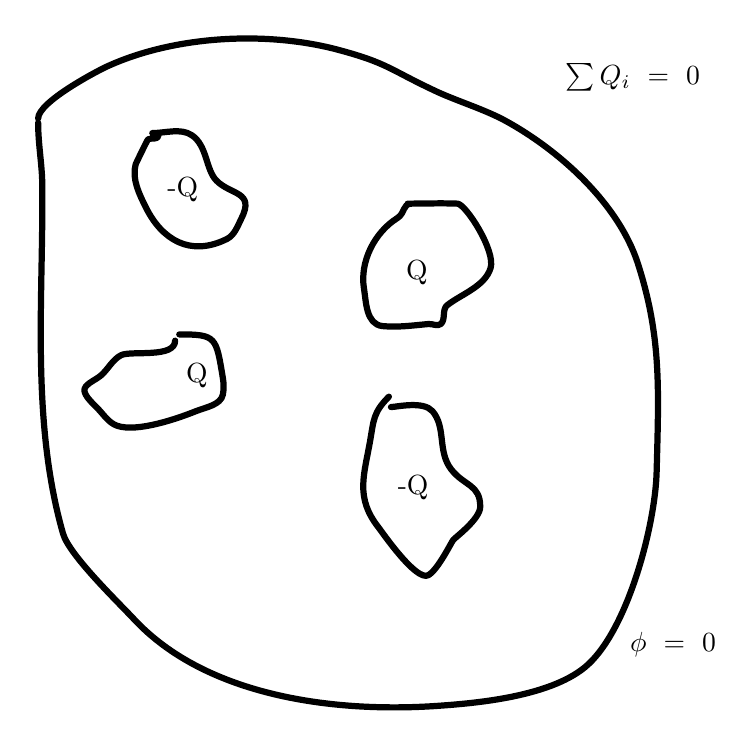
\begin{tikzpicture}[x=0.75pt,y=0.75pt,yscale=-1,xscale=1]
%uncomment if require: \path (0,300); %set diagram left start at 0, and has height of 300

%Shape: Free Drawing [id:dp13516490983958307] 
\draw  [line width=2.25] [line join = round][line cap = round] (120,134) .. controls (137.94,134) and (137.7,135.18) .. (141,155) .. controls (141.44,157.63) and (141.52,160.39) .. (141,163) .. controls (140,167.99) and (132.72,169.11) .. (128,171) .. controls (119.35,174.46) and (99.7,181.37) .. (90,178) .. controls (86.21,176.68) and (83.75,172.93) .. (81,170) .. controls (78.14,166.95) and (72.25,162.14) .. (75,159) .. controls (76.89,156.84) and (79.79,155.82) .. (82,154) .. controls (85.64,151) and (87.78,146.11) .. (92,144) .. controls (96.64,141.68) and (118,145.64) .. (118,137) ;
%Shape: Free Drawing [id:dp11119911065400023] 
\draw  [line width=2.25] [line join = round][line cap = round] (230,71) .. controls (238,71) and (246.01,70.69) .. (254,71) .. controls (257.98,71.15) and (272.49,93.69) .. (270,102) .. controls (267.32,110.93) and (255.57,114.75) .. (249,120) .. controls (246.53,121.98) and (248.43,126.98) .. (246,129) .. controls (244.46,130.28) and (241.99,128.82) .. (240,129) .. controls (232.69,129.66) and (225.31,130.7) .. (218,130) .. controls (209.92,129.23) and (210.03,118.16) .. (209,112) .. controls (206.83,98.97) and (214.17,84.77) .. (225,78) .. controls (229.03,75.48) and (227.4,71) .. (232,71) ;
%Shape: Free Drawing [id:dp8040753801936908] 
\draw  [line width=2.25] [line join = round][line cap = round] (222,169) .. controls (224.61,169) and (237.59,165.86) .. (242,171) .. controls (248.67,178.79) and (244.3,190.39) .. (251,199) .. controls (257.32,207.12) and (265,206.22) .. (265,217) .. controls (265,222.97) and (252.93,231.83) .. (252,233) .. controls (251.01,234.25) and (244.63,247.35) .. (240,250) .. controls (234.2,253.31) and (217.5,228.9) .. (216,227) .. controls (204.63,212.52) and (209.06,201.89) .. (212,185) .. controls (213.71,175.18) and (213.47,171.53) .. (221,164) ;
%Shape: Free Drawing [id:dp4629408524103269] 
\draw  [line width=2.25] [line join = round][line cap = round] (107,37) .. controls (113.34,37) and (120.72,34.48) .. (126,38) .. controls (133.59,43.06) and (132.64,54.64) .. (138,60) .. controls (144.89,66.89) and (156.46,65.08) .. (150,78) .. controls (148.18,81.64) and (146.64,86.18) .. (143,88) .. controls (125.29,96.86) and (111.65,88.31) .. (104,73) .. controls (100.99,66.97) and (96.95,59.16) .. (99,52) .. controls (99.02,51.93) and (104.56,40.27) .. (105,40) .. controls (106.46,39.12) and (110,40.47) .. (110,38) ;
%Shape: Free Drawing [id:dp12386192621787884] 
\draw  [line width=2.25] [line join = round][line cap = round] (52,30) .. controls (52,21.92) and (80.84,6.91) .. (85,5) .. controls (118.1,-10.21) and (162.68,-12.28) .. (197,-3) .. controls (220.84,3.44) and (221.12,6.32) .. (244,17) .. controls (253.44,21.41) and (267.22,25.66) .. (277,31) .. controls (302.95,45.16) and (331.64,70.88) .. (341,100) .. controls (352.33,135.25) and (351,160.42) .. (350,200) .. controls (349.35,225.83) and (336.36,275.12) .. (317,293) .. controls (300.15,308.55) and (262.9,311.71) .. (244,313) .. controls (195.54,316.3) and (133.15,308.85) .. (98,271) .. controls (90.75,263.2) and (66.94,240.28) .. (64,230) .. controls (48.46,175.59) and (54.51,117.46) .. (54,62) .. controls (53.91,52.06) and (52,42.38) .. (52,32) ;

% Text Node
\draw (122,147) node [anchor=north west][inner sep=0.75pt]   [align=left] {Q};
% Text Node
\draw (228,97) node [anchor=north west][inner sep=0.75pt]   [align=left] {Q};
% Text Node
\draw (224,201) node [anchor=north west][inner sep=0.75pt]   [align=left] {\mbox{-}Q};
% Text Node
\draw (113,57) node [anchor=north west][inner sep=0.75pt]   [align=left] {\mbox{-}Q};
% Text Node
\draw (336,276.4) node [anchor=north west][inner sep=0.75pt]    {$\phi \ =\ 0$};
% Text Node
\draw (305,2.4) node [anchor=north west][inner sep=0.75pt]    {$\sum Q_{i} \ =\ 0$};


\end{tikzpicture}
\end{center} \mbox{} \\

\noindent The potential everywhere is uniquely determined by the $Q_i$ because of
linearity $\nabla^2 \varphi$ is proportional to $\rho$ \mbox{} \\\\

In general, $\Phi_i = \sum P_{ij}Q_j$
\mbox{} \\\\

\[
  P_{ij} = \text{potential matrix} \hspace{10px} P_i \text{ is a symmetric
  matrix}
\]

\[
  \Big( Q_i \Big) = \Big( P_{ij}^{-1} \Big) \Big(\Phi_i \Big)
\]

This defines the Capacitance Matrix: 

\begin{tcolorbox}[colback = red!5!white, colframe = red!50!black, title
  = Capacitance Matrix]
  
  \[
    C_{ij} = P_{ij}^{-1}; Q_i = \sum_j C_{ij} \Phi_i
  \]
  

\end{tcolorbox} \mbox{} \\\\

\noindent \textit{ \textbf{Example}}

2 Conductor system with charge Q, -Q

%4

\begin{figure}[H]
  \centering
    \includegraphics[width = 7cm]{screenshot 170.png}
    \caption{Capacitance between two arbitrary conductors }
\end{figure}



\begin{tcolorbox}[colback = blue!5!white, colframe = blue!50!black, title
  = Capacitance]
  
  \[
  Q = C (\varphi_2 - \varphi_1) = CV
  \]
  
  

\end{tcolorbox} \mbox{} \\

\noindent \textit{ \textbf{Parallel Plate Capacitor}}

%5
\begin{figure}[H]
  \centering
    \includegraphics[width = 10cm]{screenshot 171.png}
    \caption{parallel plate capacitor}
\end{figure}


Assume a charge density $\pm \sigma$ \mbox{} \\

Gauss's Law 

\[
E(z) A = \frac{\sigma A}{\varepsilon_0} \rightarrow E(z)
= E = \frac{\sigma}{\varepsilon_0}
\] \vspace{5px} 

Potential Difference: 

\[
  \varphi(d) - \varphi(0) = -\int_0^d \vec{E} \cdot \hat{k} dz = E d
\] \vspace{5px}

Therefore, $V = E d$. If the plates have area  $A$, 

\begin{align*}
  & Q = \sigma A \\ 
  & V = \frac{\sigma}{\varepsilon}d \\\\
  & Q = \frac{\varepsilon_0 A}{d}V \\\\
  & C = \frac{\varepsilon_0 A}{d}
\end{align*}

\begin{figure}[H]
  \centering
    \includegraphics[width = 12cm]{screenshot 172.png}
    \caption{Finite sheet capacitor - fringing fields}
\end{figure}



\noindent \textit{ \textbf{Cylindrical Capacitor}}

%6
\begin{figure}[H]
  \centering
    \includegraphics[width = 14cm]{screenshot 173.png}
    \caption{cylindrical capacitor}
\end{figure}



\begin{align*}
  & E(r) A = \frac{Q}{\varepsilon} \\
  & E(r) 2\pi r l = \frac{2 \pi a l \sigma}{\varepsilon_0} \\\\
  & E(r) = \frac{\sigma}{\varepsilon_0} \frac{a}{r}
\end{align*}

\begin{align*}
  \varphi(r) - \varphi(a) &= -\int_a^r \vec{E}(r) \cdot d\vec{r} \\
                          &= -\int_a^r \frac{\sigma}{\varepsilon} \frac{a}{r}
                          dr \\
  \varphi(r) - \varphi(a) = -\frac{\sigma}{\varepsilon} a \ln \left(\frac{r}{a}
  \right) \\ 
\end{align*}

\begin{align*}
  & V = \varphi(a) - \varphi(b) \\
  & V = -\frac{\sigma}{\varepsilon}a \left[ \ln (1) - \ln (b/a) \right] \\ \\
  & V = \frac{\sigma}{\varepsilon}a\ln\left(\frac{b}{a}\right)
\end{align*}

\begin{align*}
  &\frac{Q}{l} = 2 \pi a \sigma \\
  &\frac{C}{l} = \frac{Q}{l} \frac{1}{V} = \frac{2\pi
  a \sigma}{\frac{\sigma}{\varepsilon}a \ln (b/a)} \\\\
  & \frac{C}{l} = \frac{2 \pi \varepsilon}{ \ln \left(\frac{b}{a}\right)}
\end{align*}

\end{document}
